\documentclass[11pt]{article}

\usepackage[margin=1in]{geometry}
\usepackage[american]{babel}
\usepackage[T1]{fontenc}
\usepackage{lmodern}
\usepackage{microtype}
\usepackage{graphicx}
\usepackage{booktabs}
\usepackage{caption}
\usepackage{float}
\usepackage{hyperref}
\usepackage{csquotes}

% APA7 citations via biblatex-apa (Overleaf: use biber)
\usepackage[
  backend=biber,
  style=apa,
  sortcites=true,
  sorting=nyt,
  doi=true,
  url=true
]{biblatex}
\addbibresource{references.bib}

\hypersetup{
  colorlinks=true,
  linkcolor=blue,
  citecolor=blue,
  urlcolor=blue
}

\newcommand{\PaperWordCount}{4239}

\title{Whose Goals? Cross-Cultural SDG Narratives in Multilingual News: A Scalable Pipeline and Evidence}

\author{
Sergey Volkov\textsuperscript{1}\thanks{Corresponding author: \href{mailto:sergey.volkov@connect.hku.hk}{sergey.volkov@connect.hku.hk}} \quad
HU Saliushuang\textsuperscript{1}\thanks{\href{mailto:sandyhu623@outlook.com}{sandyhu623@outlook.com}} \quad
Chengbin Zhou\textsuperscript{1}\thanks{\href{mailto:chengbin.zhou@connect.hku.hk}{chengbin.zhou@connect.hku.hk}}\\
\textsuperscript{1}The University of Hong Kong, Hong Kong SAR, China
}

\date{EMCSDG 2026 (Hong Kong, March 27--28, 2026)}

\begin{document}
\maketitle

\begin{abstract}
Cross-cultural progress on the United Nations Sustainable Development Goals (SDGs) depends not only on policy, but also on how the goals are communicated and legitimized in everyday media ecosystems. We present a scalable, reproducible multilingual pipeline that retrieves global digital news from GDELT, applies weakly supervised SDG tagging via multilingual keyword patterns, and supports comparative analysis by time and language community. On a full 2024--2025 corpus (495{,}520 retrieved records; 158{,}647 SDG-labeled articles), we obtain 182{,}719 article--SDG mentions (mean 1.15 SDGs/article) with a strongly skewed agenda: SDG~17 accounts for 59.3\% of mentions, followed by SDG~3 (10.0\%) and SDG~7 (3.6\%). We strengthen novelty by quantifying \emph{cross-language agenda divergence}: for the top 10 languages by volume, we compute SDG distributions over all 17 goals and pairwise Jensen--Shannon divergence (JSD), finding substantial variation (JSD range 0.01--0.26) and large differences in SDG portfolio diversity (effective number of SDGs $\approx$ 1.2--8.3). We also operationalize \emph{punctuated attention} via a transparent monthly spike detector (z-scores over 24 months), identifying high-signal spike months such as SDG~5 (Mar~2024), SDG~15 (Oct~2024), SDG~10 (Jan~2025), and SDG~14 (Jun~2025). A pilot semantic-framing layer (embeddings $\rightarrow$ clustering $\rightarrow$ JSD over ``frame family'' distributions) is retained as supporting evidence. We discuss threats to measurement equivalence (query bias, language imbalance, and keyword sensitivity) and outline a validation protocol using supervised SDG corpora (OSDG-CD and SDGi). Contributions: (1) an end-to-end multilingual SDG media monitoring pipeline; (2) language-level agenda divergence and diversity metrics; and (3) a reproducible spike analysis for temporal SDG attention dynamics.
\end{abstract}

\noindent\textbf{Keywords:} SDG 17; SDG 10; multilingual news; GDELT; cross-lingual semantic framing; SDG tagging

\section{Introduction}
The SDGs constitute a globally shared framework for sustainable and inclusive development, yet their societal effectiveness depends on how the goals become visible, meaningful, and legitimate within public communication. Digital news---distributed via online platforms and indexed by global monitoring projects---is a key ``emerging media'' layer through which SDG-related narratives circulate and are contested. Comparative research suggests that sustainability-related media agendas vary substantially across regions rather than following a single global pattern \parencite{barkemeyer2013sustainability}, while world-news monitoring reports overall low SDG visibility and strong cross-regional differences in tone and attention \parencite{czvetko2021intertwining}. These findings motivate a multilingual, cross-cultural approach that can quantify \emph{what} SDG topics become salient and begin to characterize \emph{how} they are framed across language communities.

We ask: \emph{Whose goals} become visible in multilingual news, and which goals or populations may be underrepresented when global SDG discourse is dominated by particular languages and institutional frames? Addressing this question at scale requires (i) a global news source with consistent metadata, (ii) a transparent SDG labeling approach that can be audited for bias, and (iii) a cross-lingual framing representation that supports comparability across languages. This paper contributes an end-to-end pipeline that links these components, producing camera-ready figures and tables for full-corpus trends (2024--2025) and a pilot semantic-framing analysis.

We focus on three research questions (RQs):
\begin{enumerate}
  \item \textbf{RQ1 (Agenda distribution):} Which SDGs receive the most attention in multilingual news, and how does the SDG distribution differ across language communities?
  \item \textbf{RQ2 (Narratives over time):} How does SDG-related attention evolve over time, and which goals exhibit punctuated (event-driven) versus relatively stable coverage?
  \item \textbf{RQ3 (Measurement equivalence):} What biases arise from keyword-based SDG tagging in multilingual corpora, and how can supervised datasets improve cross-language comparability?
\end{enumerate}

Our primary empirical contribution is descriptive evidence over a full 2024--2025 corpus, complemented by a clearly labeled pilot semantic-framing subset that demonstrates a scalable approach to cross-lingual narrative comparison.

\section{Related Work}
Research on sustainability communication consistently finds cross-national differences in issue salience and agenda structure. Early comparative work shows that sustainability-related media coverage varies by region and correlates with socioeconomic development \parencite{barkemeyer2013sustainability}. More recent large-scale monitoring that maps world news to SDGs likewise reports low overall SDG visibility and substantial regional differences in tone and attention \parencite{czvetko2021intertwining}. These findings motivate scalable methods that can support multilingual, cross-cultural comparisons rather than single-language analyses.

\textbf{Global news monitoring and GDELT.} GDELT is widely used in computational social science and communication research because it provides global-scale news metadata with time and language fields and APIs for large-scale retrieval \parencite{leetaru2013gdelt,gdelt2015gkgcodebook,hopp2019icore}. However, using GDELT for substantive inference requires careful attention to sampling (query design), source coverage, and the limited textual fields available at scale (titles/snippets), especially when comparing languages.

\textbf{SDG text classification and tagging.} SDG-related text classification has been approached via weak supervision (keyword lists), supervised learning on labeled corpora, and more recently instruction-tuned language models \parencite{pukelis2022osdg20,fankhauser2024sdgllm}. Open labeled datasets such as OSDG-CD and SDGi enable supervised multilingual SDG classification and cross-language validation \parencite{osdgcd2022,skrynnyk2024sdgi,undp2024sdgi}. In this paper, we use transparent keyword-based SDG tagging as a baseline that is fast and auditable, while explicitly treating measurement equivalence as a research problem (RQ3) rather than an assumption.

\textbf{Cross-lingual framing and divergence.} To operationalize cross-cultural narrative differences, we use a semantic-framing layer based on multilingual sentence embeddings \parencite{reimers2019sbert}, a 2D projection for visualization (UMAP where available) \parencite{mcinnes2018umap}, and clustering to approximate recurring lexical ``frame families'' (k-means) \parencite{macqueen1967kmeans}. We quantify cross-language differences using Jensen--Shannon divergence (JSD) between language-specific cluster distributions \parencite{lin1991jsd}. As a robustness fallback, the pipeline can also use TF--IDF representations \parencite{salton1988term} and truncated SVD/LSA embeddings \parencite{deerwester1990indexing} if neural embeddings are unavailable.

\textbf{Regional and topic-modeling baselines.} Beyond global monitoring, work has also examined SDG coverage in specific regional media ecosystems using AI/NLP approaches \parencite{alsuhaibani2025ai}. Topic models such as Latent Dirichlet Allocation (LDA) remain common baselines for summarizing large corpora \parencite{blei2003lda}, but require careful multilingual preprocessing and validation when used for cross-language comparison.

\section{Data}
\subsection{Source and retrieval}
We use GDELT as the primary source of global digital news metadata and text snippets \parencite{leetaru2013gdelt,gdelt2015gkgcodebook}. Collection is implemented via windowed GDELT DOC queries (90-day windows) over the UTC interval 2024-01-01 to 2025-12-31.\footnote{Query string (as implemented in \texttt{reports/01\_gdelt\_collection\_report\_2024\_2025.json}): (\texttt{"sustainable development"} OR \texttt{"sustainable development goals"} OR \texttt{"climate change"} OR \texttt{"global warming"} OR \texttt{"renewable energy"} OR \texttt{"public health"} OR \texttt{poverty} OR \texttt{inequality} OR \texttt{biodiversity} OR \texttt{SDG} OR \texttt{SDGs}).}
Across 2024--2025, the pipeline retrieves 495{,}520 records, each associated with a unique URL in this collection (i.e., URL-based deduplication does not reduce the corpus further in this particular run; Table~\ref{tab:corpus_stats}). The analysis text used for SDG tagging is constructed as \texttt{title + ". " + snippet} for each record.

\subsection{Preprocessing and pilot subset}
We apply text-quality filters to remove empty or low-information records and then assign SDG labels (multi-label) using multilingual keyword patterns (Section~\ref{sec:methods:tagging}). The resulting full-corpus dataset contains 158{,}647 SDG-labeled articles and 182{,}719 article--SDG mentions (Table~\ref{tab:corpus_stats}).

To validate the end-to-end methodology and enable richer semantic framing with manageable computational cost, we also analyze a three-month pilot subset. When the pilot window cannot be recovered from cached subset metadata, we define it as the first 90-day window starting 2024-01-01 UTC (Jan--Mar 2024). The pilot collection contains 56{,}000 deduplicated records and yields 17{,}795 SDG-labeled articles and 20{,}782 article--SDG mentions (reported in the extended abstract text in this repository).

\begin{table}[H]
\centering
\caption{Corpus statistics for the full 2024--2025 dataset (GDELT retrieval, SDG tagging, and derived mention counts).}
\label{tab:corpus_stats}
\begin{tabular}{lrrrrr}
\toprule
Scope & Raw records & SDG-labeled articles & Article--SDG mentions & Mean SDGs/article & UTC span \\
\midrule
Full 2024--2025 & 495{,}520 & 158{,}647 & 182{,}719 & 1.15 & 2024-01-01 to 2025-12-31 \\
\bottomrule
\end{tabular}
\end{table}

\section{Methods}
\label{sec:methods}
\subsection{Pipeline overview}
Figure~\ref{fig:pipeline} summarizes the pipeline from retrieval through descriptive aggregation and pilot semantic framing.

\begin{figure}[H]
\centering
\small
\setlength{\fboxsep}{6pt}
\setlength{\tabcolsep}{4pt}
\renewcommand{\arraystretch}{1.15}
\begin{tabular}{c c c c c}
\fbox{\parbox{0.18\linewidth}{\centering GDELT retrieval\\(windowed queries,\\2024--2025)}} &
$\rightarrow$ &
\fbox{\parbox{0.20\linewidth}{\centering Text construction\\\& filtering\\(title+snippet)}} &
$\rightarrow$ &
\fbox{\parbox{0.20\linewidth}{\centering Weakly supervised\\SDG tagging\\(keyword patterns)}} \\
\\[-2pt]
\multicolumn{5}{c}{$\swarrow$ \hspace{9.5em} $\searrow$} \\
\\[-2pt]
\fbox{\parbox{0.26\linewidth}{\centering Pilot semantic framing\\(embeddings $\rightarrow$ clustering\\$\rightarrow$ JSD)}} &
\multicolumn{3}{c}{} &
\fbox{\parbox{0.26\linewidth}{\centering Aggregation \& summaries\\(monthly trends;\\language/country)}} \\
\\[-2pt]
\multicolumn{5}{c}{$\downarrow$} \\
\multicolumn{5}{c}{\fbox{\parbox{0.62\linewidth}{\centering Camera-ready paper figures \& tables}}} \\
\end{tabular}
\caption{Scalable multilingual pipeline for SDG narrative monitoring and pilot cross-lingual framing. Full-corpus aggregation runs on 2024--2025 data; semantic framing is reported as a pilot subset analysis.}
\label{fig:pipeline}
\end{figure}

\subsection{Weakly supervised SDG tagging}
\label{sec:methods:tagging}
We implement multi-label SDG tagging via multilingual keyword matching. For each SDG, we compile a set of goal-relevant keywords into case-insensitive regular expressions (stored in \texttt{sdg\_keywords.json} in this repository). A document is assigned all SDGs whose patterns match the document text. Each assigned SDG contributes one \emph{article--SDG mention}; multi-label documents therefore contribute multiple mentions. This baseline is fast and transparent but is expected to exhibit language-dependent sensitivity and polysemy errors, motivating validation (Section~\ref{sec:validity}).

\subsection{Aggregation and descriptive summaries}
For full-corpus descriptive analysis, we aggregate article--SDG mentions by month (UTC) and compute overall SDG shares (Table~\ref{tab:sdg_counts_full}) and monthly volume trends (Figure~\ref{fig:mentions_over_time}).

\subsection{Language agenda divergence and portfolio diversity}
To quantify how SDG agendas differ across language communities, we represent each language's agenda as a probability distribution over all 17 SDGs and compute pairwise Jensen--Shannon divergence (JSD) for the top 10 languages by mention volume \parencite{lin1991jsd}. We complement divergence with portfolio diversity metrics: Shannon entropy $H=-\sum_s p(s)\log p(s)$ and the effective number of SDGs $\exp(H)$ (Table~\ref{tab:lang_diversity}).

\subsection{Temporal spike detection (punctuated attention)}
To operationalize punctuated attention (RQ2), we aggregate monthly SDG mention counts over the 24-month window (2024-01 to 2025-12) and compute within-SDG z-scores $z=(x-\mu)/\sigma$. We flag a month as a spike event if $z\ge 2.5$, the monthly count is at least 50 mentions, and the SDG has at least 1{,}000 mentions over the full period; we then summarize spikes with top contributing languages and source countries (Appendix Table~\ref{tab:spike_events}).

\subsection{Pilot semantic framing and cross-language divergence (supporting)}
To move from ``how much'' to ``how framed,'' we retain a pilot semantic-framing layer on a three-month subset. We embed pilot documents using multilingual sentence embeddings (Sentence-BERT / sentence-transformers; \cite{reimers2019sbert}), cluster in embedding space with k-means ($k=60$) \parencite{macqueen1967kmeans}, and compute JSD over language-specific cluster distributions \parencite{lin1991jsd}. We report pilot clusters and divergence as supporting tables (Appendix Tables~\ref{tab:clusters} and \ref{tab:jsd_pairs}) and treat them as exploratory.

\section{Results}
\subsection{Full 2024--2025 corpus: agenda distributions and trends}
Table~\ref{tab:sdg_counts_full} reports the top SDGs by mention count in the full 2024--2025 corpus. SDG~17 (Partnerships for the Goals) dominates with 108{,}281 mentions (59.3\%), consistent with the interpretation that SDG discourse in news is frequently framed through cooperation, funding, and international coordination narratives. SDG~3 (Good Health and Well-Being) is second (18{,}188; 10.0\%), followed by SDG~7 (Affordable and Clean Energy; 6{,}516; 3.6\%) and SDG~13 (Climate Action; 6{,}336; 3.5\%).

\begin{table}[H]
\centering
\caption{Top SDG mention counts and shares in the full 2024--2025 corpus (182{,}719 article--SDG mentions).}
\label{tab:sdg_counts_full}
\begin{tabular}{lrr}
\toprule
SDG & Mentions & Share \\
\midrule
SDG 17 (Partnerships) & 108{,}281 & 59.3\% \\
SDG 3 (Health) & 18{,}188 & 10.0\% \\
SDG 7 (Clean energy) & 6{,}516 & 3.6\% \\
SDG 13 (Climate) & 6{,}336 & 3.5\% \\
SDG 4 (Education) & 5{,}835 & 3.2\% \\
SDG 1 (No poverty) & 4{,}696 & 2.6\% \\
SDG 8 (Decent work) & 4{,}557 & 2.5\% \\
SDG 9 (Industry/innovation) & 4{,}378 & 2.4\% \\
SDG 6 (Clean water) & 4{,}281 & 2.3\% \\
SDG 5 (Gender equality) & 4{,}052 & 2.2\% \\
Other SDGs (combined) & 15{,}599 & 8.5\% \\
\bottomrule
\end{tabular}
\end{table}

Figure~\ref{fig:mentions_over_time} shows monthly SDG mention volume over 2024--2025. The series exhibits punctuated peaks and troughs rather than a monotonic trend, consistent with event-driven attention dynamics (RQ2). The plot is restricted to the 2024--2025 window to avoid out-of-range month artifacts.

\begin{figure}[H]
\centering
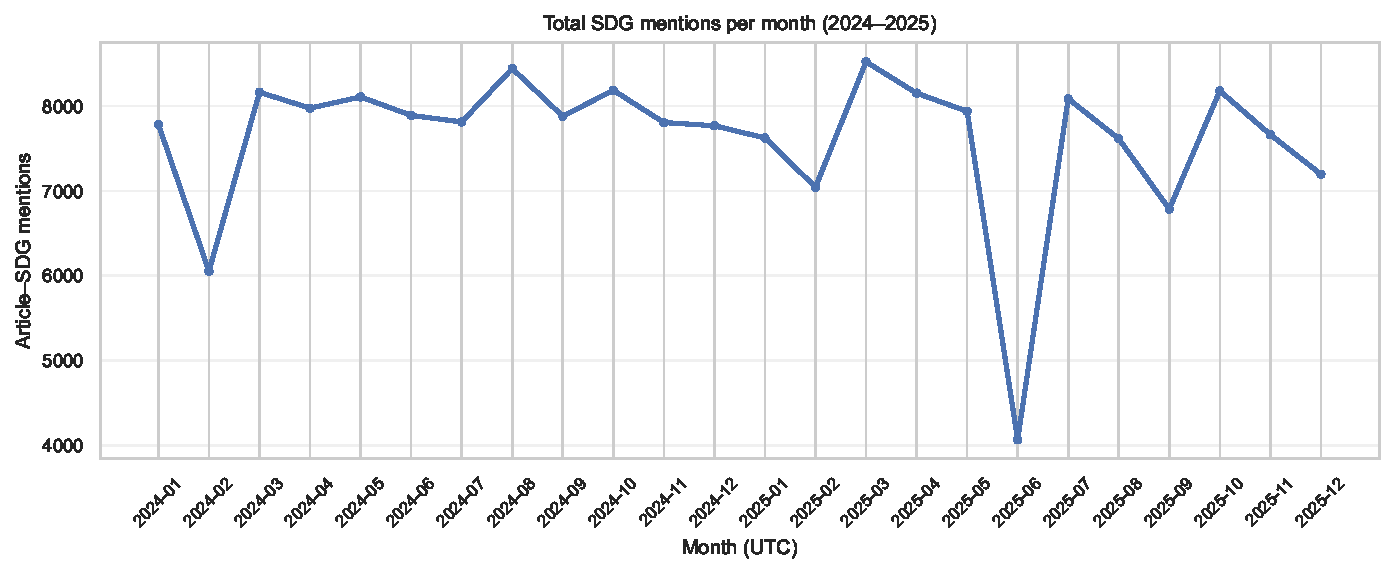
\includegraphics[width=\linewidth]{figures/fig02_total_mentions_per_month.pdf}
\caption{Total SDG mentions per month in 2024--2025 (article--SDG mentions aggregated by UTC month).}
\label{fig:mentions_over_time}
\end{figure}

\subsection{Cross-language agenda divergence and portfolio diversity}
Language distributions are highly imbalanced: English accounts for 109{,}585 mentions (60.0\%) and Spanish for 32{,}276 (17.7\%), followed by German (5.6\%) and French (4.0\%). We quantify \emph{agenda divergence} between language communities by computing pairwise JSD over SDG distributions for the top 10 languages (Figure~\ref{fig:lang_jsd}). Divergence is non-trivial (JSD range 0.01--0.26): Chinese is the most divergent agenda among the top languages (e.g., Turkish--Chinese JSD $\approx 0.26$; German--Chinese $\approx 0.26$), while several European-language pairs are closely aligned (e.g., Italian--Romanian $\approx 0.01$).

\begin{figure}[H]
\centering
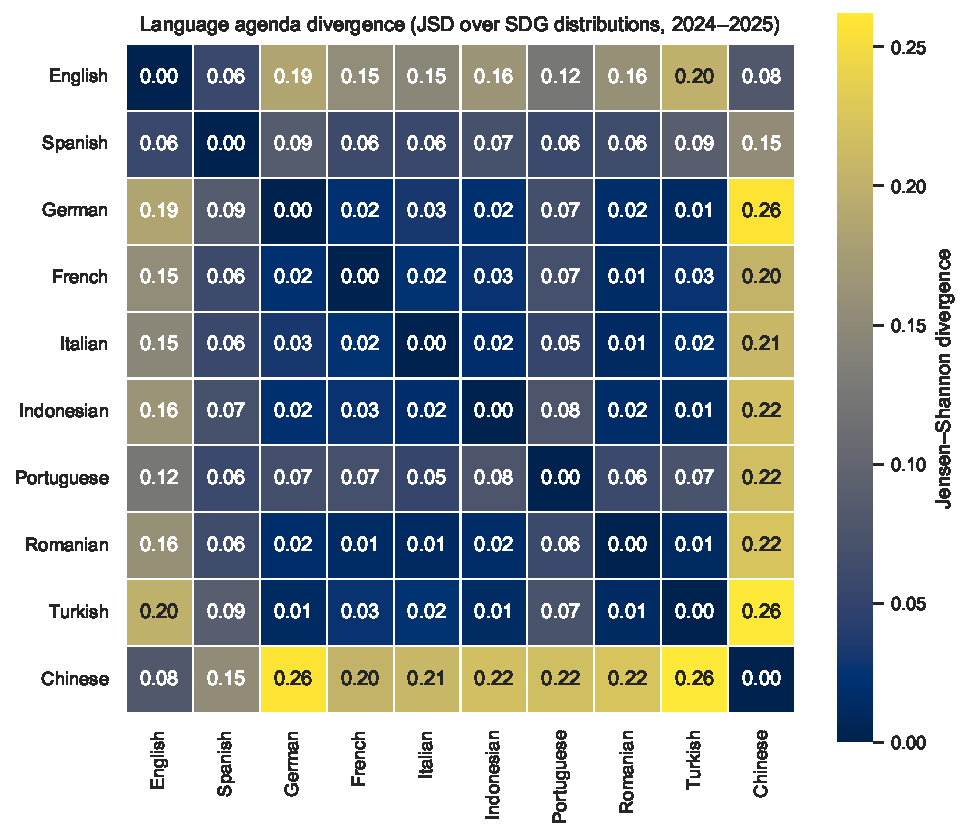
\includegraphics[width=0.92\linewidth]{figures/fig03_language_sdg_jsd_heatmap.pdf}
\caption{Language agenda divergence (JSD) over SDG distributions for the top 10 languages by mention volume (full 2024--2025 corpus).}
\label{fig:lang_jsd}
\end{figure}

Agenda divergence is mirrored by strong differences in \emph{portfolio diversity} (Table~\ref{tab:lang_diversity}). Several languages are extremely concentrated in SDG~17 (e.g., German, Turkish), while English and Chinese exhibit substantially broader SDG portfolios (effective SDGs $>7$). Notably, SDG~10 remains a low-share topic across the top languages (highest share among the top languages: Portuguese, 4.9\%), reinforcing the paper's ``Whose goals?'' concern about inequality narratives being crowded out when partnership framing dominates.

\begin{table}[H]
\centering
\caption{SDG portfolio diversity by language (top languages; full 2024--2025 corpus).}
\label{tab:lang_diversity}
\begin{tabular}{lrrrrr}
\toprule
Language & Mentions & SDG17 share & SDG10 share & Entropy & Eff. SDGs \\
\midrule
English & 109,585 & 46.0\% & 1.1\% & 2.03 & 7.64 \\
Spanish & 32,276 & 70.5\% & 0.9\% & 1.28 & 3.59 \\
German & 10,281 & 95.4\% & 0.7\% & 0.28 & 1.33 \\
French & 7,372 & 90.2\% & 0.7\% & 0.54 & 1.72 \\
Italian & 5,628 & 88.0\% & 0.0\% & 0.62 & 1.86 \\
Indonesian & 3,137 & 92.8\% & 0.0\% & 0.41 & 1.50 \\
Portuguese & 2,814 & 74.7\% & 4.9\% & 1.09 & 2.96 \\
Romanian & 2,190 & 92.5\% & 0.0\% & 0.43 & 1.54 \\
Turkish & 1,361 & 97.0\% & 0.0\% & 0.19 & 1.20 \\
Chinese & 1,320 & 35.5\% & 0.3\% & 2.12 & 8.33 \\
\bottomrule
\end{tabular}
\end{table}


\subsection{Temporal spikes (punctuated attention)}
Figure~\ref{fig:spike_heatmap} visualizes punctuated attention by plotting monthly z-scores (within-SDG) for a focused set of SDGs; outlined cells indicate detected spikes using a transparent threshold rule ($z\ge 2.5$, monthly mentions $\ge 50$, SDG total $\ge 1{,}000$). Under these strict criteria, only a small number of SDG-months qualify as spikes (Appendix Table~\ref{tab:spike_events}), providing an interpretable shortlist of event-driven attention surges.

\begin{figure}[H]
\centering
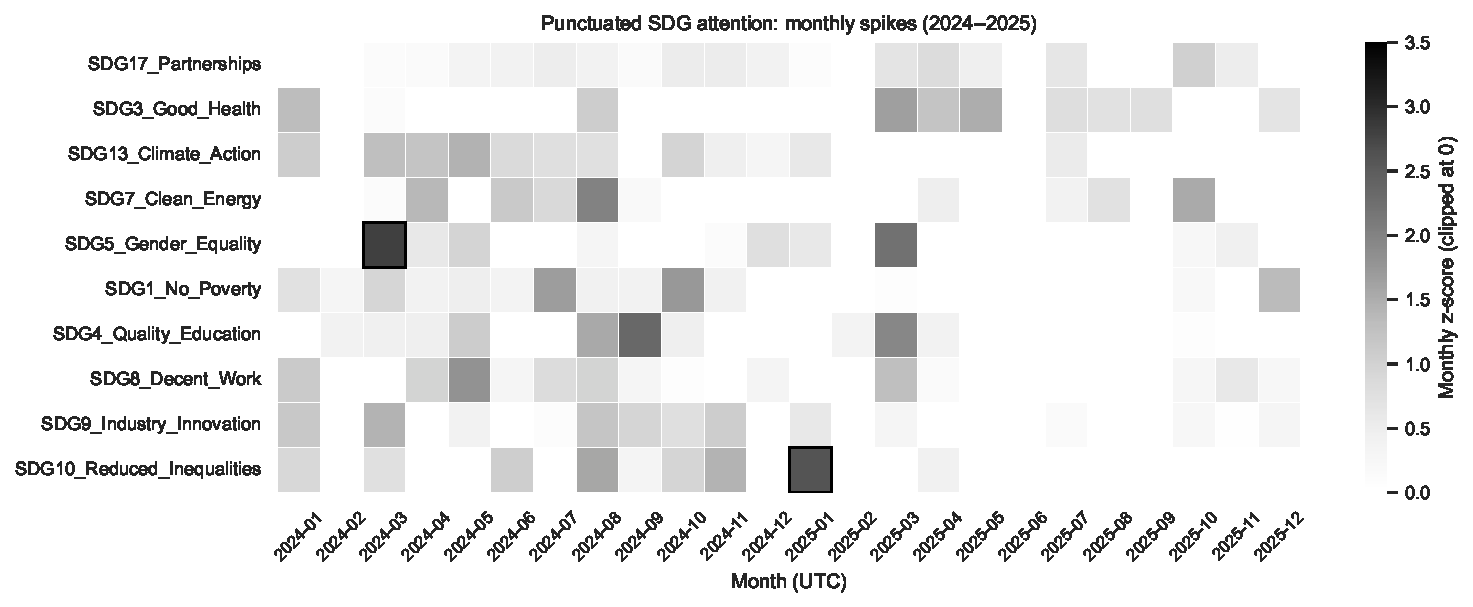
\includegraphics[width=\linewidth]{figures/fig04_sdg_spike_heatmap.pdf}
\caption{Temporal spike heatmap for selected SDGs (2024--2025). Values are monthly z-scores (clipped at 0); outlined cells mark detected spike months under the paper's threshold rule.}
\label{fig:spike_heatmap}
\end{figure}

\subsection{Pilot semantic framing (supporting)}
We retain a pilot semantic-framing layer on a three-month subset (Jan--Mar 2024) to illustrate how framing can be compared beyond SDG volumes. The pilot subset contains 17{,}795 SDG-labeled articles and 20{,}782 article--SDG mentions (mean 1.17 SDGs/article), again dominated by SDG~17 (56.4\%). Clustering over multilingual embeddings yields recurring lexical ``frame families'' (Appendix Table~\ref{tab:clusters}) and language-pair divergences over cluster distributions (Appendix Table~\ref{tab:jsd_pairs}). We treat these framing results as exploratory and prioritize full-corpus, distributional metrics for robust cross-cultural comparison.

\section{Robustness, Bias, and Validity}
\label{sec:validity}
Our measurements reflect a chain of assumptions that can affect cross-cultural inference.

\textbf{Retrieval and source bias.} Query design shapes which documents enter the corpus; SDG-related language may be expressed without explicit ``SDG'' terminology, and the availability of sources varies across languages and regions in GDELT. URL-based ``deduplication'' may not remove near-duplicates with different URLs.

\textbf{Text limitations.} The pipeline uses \texttt{title+snippet} text fields for scalability. Snippets can be short, templated, or uneven across sources, which can inflate generic clusters and reduce framing specificity.

\textbf{Keyword-tagging bias.} Keyword patterns differ in sensitivity across languages and can produce false positives (polysemy) and false negatives (missing synonyms). These biases can also shift apparent SDG portfolios by language even if substantive agendas are closer.

\textbf{Semantic framing limitations.} Embedding models and 2D projections can introduce language- and domain-specific artifacts. Cluster interpretability is approximate and should be treated as exploratory.

\textbf{Light validation protocol (planned).} To support RQ3, we provide a validation plan that (i) exports a stratified sample for manual coding across languages and SDGs, and (ii) compares the keyword baseline to supervised multilingual SDG taggers trained on OSDG-CD and SDGi \parencite{osdgcd2022,skrynnyk2024sdgi,undp2024sdgi}. At the time of writing, manual labels are not yet available for reporting precision/recall; we therefore treat validation outcomes as ongoing work and emphasize transparency and reproducibility.

\section{Discussion}
The 2024--2025 results reveal a highly skewed SDG news agenda dominated by SDG~17 (Partnerships). This dominance is substantively meaningful for ``Whose goals?'' because institutional partnership language can crowd out coverage of distributional harms and inequality-related narratives (SDG~10) unless explicitly foregrounded. Beyond volume, the language-agenda analysis shows that multilingual news does not simply scale the same SDG portfolio across languages: pairwise JSD reveals substantial divergence for some language communities, while others are closely aligned. Portfolio diversity metrics further indicate that some languages discuss SDGs through an extremely concentrated lens (SDG~17 shares $>90\%$), whereas English and Chinese distribute attention across a much broader set of goals. Finally, spike detection provides a compact, reproducible map of event-driven SDG salience---a shortlist of months where attention to specific goals sharply departs from their typical baselines---that can guide targeted qualitative follow-up and validation.

\section{Conclusion}
We presented a reproducible multilingual pipeline for monitoring SDG-related narratives in global digital news and reported full-corpus descriptive results for 2024--2025 alongside supporting pilot semantic framing. The paper contributes (i) quantitative language-level agenda divergence (JSD) and portfolio diversity metrics, and (ii) a transparent spike detector for punctuated SDG attention dynamics. Together, these results highlight strong agenda skew (SDG~17 dominance), systematic cross-language differences in SDG portfolios, and a small set of interpretable spike months suitable for follow-up qualitative analysis. Future work will (i) train and validate supervised multilingual SDG classifiers using OSDG-CD and SDGi, (ii) extend framing analysis with robust cross-lingual representations and evaluation, and (iii) integrate actor and co-mention networks to better characterize how partnerships, inequalities, and policy debates are communicated across contexts.

\section*{Code and Data Availability}
Project repository: \url{https://github.com/nZiben/sdg-multilingual-media-narratives}

\printbibliography

\appendix
\renewcommand{\thetable}{A\arabic{table}}
\setcounter{table}{0}

\section{Appendix: Supplementary Tables (tables only)}

\begin{table}[H]
\centering
\caption{Top SDG$\times$country co-occurrence edges (full corpus; extracted from the analysis notebook output).}
\label{tab:top_edges}
\begin{tabular}{llr}
\toprule
Country & SDG & Weight \\
\midrule
United States & SDG 17 & 22{,}453 \\
Spain & SDG 17 & 9{,}762 \\
United States & SDG 3 & 8{,}378 \\
Germany & SDG 17 & 7{,}960 \\
United Kingdom & SDG 17 & 6{,}670 \\
Italy & SDG 17 & 4{,}773 \\
Argentina & SDG 17 & 3{,}925 \\
Canada & SDG 17 & 3{,}704 \\
India & SDG 17 & 3{,}306 \\
France & SDG 17 & 3{,}108 \\
Australia & SDG 17 & 2{,}927 \\
Indonesia & SDG 17 & 2{,}918 \\
Mexico & SDG 17 & 2{,}584 \\
United States & SDG 4 & 2{,}506 \\
United States & SDG 13 & 2{,}456 \\
\bottomrule
\end{tabular}
\end{table}

\begin{table}[H]
\centering
\caption{Detected monthly spike events in SDG attention (full corpus; z-score thresholding).}
\label{tab:spike_events}
\begin{tabular}{llrrp{0.28\linewidth}p{0.28\linewidth}}
\toprule
Month & SDG & Mentions & $z$ & Top languages & Top countries \\
\midrule
2025-06 & SDG14\_Life\_Below\_Water & 197 & 3.93 & english (118); spanish (33); portuguese (20) & United States (53); Australia (13); Portugal (11) \\
2024-10 & SDG15\_Life\_On\_Land & 276 & 2.82 & english (164); spanish (91); italian (8) & United States (77); Colombia (25); Spain (21) \\
2024-03 & SDG5\_Gender\_Equality & 342 & 2.79 & english (290); spanish (27); portuguese (8) & United States (88); United Kingdom (37); Australia (27) \\
2025-01 & SDG10\_Reduced\_Inequalities & 130 & 2.58 & english (116); russian (4); german (3) & United States (55); Australia (39); India (5) \\
\bottomrule
\end{tabular}
\end{table}


\begin{table}[H]
\centering
\caption{Pilot semantic ``frame families'' (clusters) from \texttt{data/processed/04\_cluster\_terms.csv}; top clusters by size.}
\label{tab:clusters}
\begin{tabular}{r r p{0.62\linewidth}}
\toprule
Cluster & $n$ & Example top terms \\
\midrule
9 & 4{,}742 & new; news; poverty; 2024; united; says; school; united kingdom; women; hospital; report \\
4 & 1{,}022 & new; calls; women; 2024; funding; solar; council; education; county; school; kids \\
2 & 1{,}016 & state; state union; address; women; 2024; poverty; biden; president; future \\
5 & 972 & 2024; county; women; india; poverty; schools; global; children \\
23 & 935 & world; united; country; industry; women; 2024; states; poverty \\
26 & 769 & public health; health care; mental health; measles; emergency; officials \\
58 & 572 & climate change; heat; impact; farmers; fight; world \\
\bottomrule
\end{tabular}
\end{table}

\begin{table}[H]
\centering
\caption{Pilot language-pair divergence (JSD over cluster distributions). Top and bottom pairs are computed over the languages included in the pilot JSD output.}
\label{tab:jsd_pairs}
\begin{tabular}{lr}
\toprule
\multicolumn{2}{c}{Highest JSD pairs} \\
\midrule
\texttt{roman}--\texttt{alban} & 0.693 \\
\texttt{chine}--\texttt{catal} & 0.693 \\
\texttt{catal}--\texttt{finni} & 0.693 \\
\texttt{alban}--\texttt{catal} & 0.693 \\
\texttt{roman}--\texttt{greek} & 0.693 \\
\midrule
\multicolumn{2}{c}{Lowest JSD pairs} \\
\midrule
\texttt{chine}--\texttt{finni} & 0.026 \\
\texttt{chine}--\texttt{croat} & 0.054 \\
\texttt{finni}--\texttt{croat} & 0.070 \\
\texttt{en}--\texttt{hi} & 0.088 \\
\texttt{chine}--\texttt{turki} & 0.107 \\
\bottomrule
\end{tabular}
\end{table}

\bigskip
\noindent\textit{Word count (approx., including abstract and references): \PaperWordCount.}

\end{document}
